\chapter{Perancangan}
\label{chap:perancangan}

Pada bab ini akan dibahas perancangan dari perangkat lunak mulai dari perancangan antarmuka, dan perancangan untuk algoritma setiap \textit{route} yang dipakai. 

\section{Perancangan Routing Handler}
\subsection{\textit{Route} /}
Pada \textit{route} ini, akan memiliki kalimat pengantar dan juga sebuah tombol yang bisa membawa pengguna untuk melakukan \textit{login} kepada ``\textit{Windows Live}''. Tombol itu akan membawa pengguna kepada halaman untuk melakukan \textit{login} Windows Live dan juga setelah \textit{login}, program akan meminta izin untuk bisa mendapatkan data mengenai \textit{event} yang terdapat pada kalender pengguna.

\subsection{\textit{Route} /authorize}
\textit{Route} ini akan muncul ketika langkah dari \textit{route} / sudah selesai dijalankan sehingga \textit{access token} dan izin dari pengguna sudah didapatkan oleh program ini. Di \textit{route} ini akan ada kalimat penjelasan untuk halaman ini dan juga ada tombol untuk pengguna bisa melakukan \textit{login} pada aplikasi \textit{Slack} untuk didapatkan \textit{access token} dan izinnya juga. Setelah tombol itu ditekan oleh pengguna, maka tombol itu akan mengantarkan pengguna kepada halaman untuk mengisi \textit{workspace} yang dipakai oleh pengguna dan juga akun yang dipakai oleh pengguna untuk melakukan sinkronisasi dengan \textit{Outlook Calendar}. Setelah melakukan \textit{login}, maka akan tampil halaman untuk pengguna memberikan izin kepada program untuk bisa mengubah data termasuk status pengguna di dalam aplikasi \textit{Slack}. 

\subsection{\textit{Route} /slackAuthorize}
\textit{Route} ini hanya menampilkan konfirmasi yang didapat dari hasil perekaman data dari \textit{Slack} yang berupa \textit{access token} dari aplikasi tersebut. 

\subsection{\textit{Route} /statusChanger}
\textit{Route} ini yang berfungsi mengeksekusi pengambilan data dari \textit{Outlook Calendar} secara berkala, dan jika ada data \textit{event} yang sesuai dengan waktu sekarang, maka lewat \textit{route} ini juga program ini akan mengganti status pada aplikasi \textit{Slack}. Sebelum melakukan pengambilan data pada \textit{Outlook Calendar}, pada \textit{route} ini juga melakukan pengecekan pada \textit{access token} yang didapat pada saat awal melakukan \textit{login Windows Live}. Jika \textit{access token} yang terekam pada \textit{database} sudah kadaluarsa, maka melalui \textit{route} ini juga program akan meminta \textit{access token} yang baru untuk bisa mengambil data \textit{event} dari \textit{Outlook Calendar}. Adapun pseudocode yang dirancang adalah seperti\\
\\

\begin{lstlisting}[caption={Pseudocode untuk /statusChanger}, label={code:pseudocode_statusChanger}]
do connection to database. 

router.get(/, function(){
    timestampNow=new Date()
    
    client.query("SELECT * FROM public.Credentials", (err,res)=>{
        for each res dari hasil query
            check masa kadaluarsa dari access token per row
            if(expired){
                minta ulang dengan refresh token memakai
                function useRefreshToken()
                
                mendapatkan event dengan memakai access
                token yang baru memakai function getEvent()
            }
            else{
                mendapatkan event dengan memakai access
                token yang lama memakai function getEvent()
            }
    })
})

async function getEvent(accessToken, slackAccessToken){
    result=mengirimkan request /me/events
    
    for each result{
        if(timestampNow>=startTime&&timestampNow<=endTime){
            panggil function changeStatusSlack()
        }
        else{
            tidak melakukan apa apa. 
        }
    }
}

async function useRefreshToken(refresh_token){
    melakukan request menggunakan refresh token
    
    menyimpan data yang diperlukan kembali ke dalam tabel 
    
    return newToken
}

async function changeStatusSlack(slack_access_token, endTime){
    mengirimkan request dengan menggunakan slack access token
    ditambah dengan parameter status_expiration diisi dengan endtime
}

\end{lstlisting}

\section{Perancangan \textit{Helper}}
\subsection{auth.js}
Pada \textit{file javascript} ini, terdapat kode yang membantu untuk melakukan \textit{request} untuk mendapatkan \textit{access token} dari \textit{Microsoft Graph} maupun dari \textit{Slack}. Cara mendapatkan \textit{access token} di file ini dengan cara menggunakan \textit{library simple oauth2} yang membantu untuk melakukan \textit{request} ke aplikasi yang akan dituju. Selain untuk meminta \textit{akses token}, di dalam file ini juga berisi kode yang membantu program ini agar \textit{access token} dan data yang dibutuhkan lainnya disimpan di dalam basis data. Pada \textit{helper} ini terdapat konstanta dan juga fungsi-fungsi seperti:
\begin{itemize}
    \item \textit{Constanta}
    \begin{itemize}
        \item \textbf{\{Client\}}: Konstanta ini merupakan konstanta yang memanggil \textit{library} dari \textit{postgres}. \textit{Postgres} merupakan jenis basis data yang dipakai di dalam program ini. 
        \item \textbf{client}: Konstanta yang menginisialisasi kelas \textit{Client} yang dipanggil dari konstanta sebelumnya. Konstanta ini menginisialisasi kelas \textit{Client} dengan parameter \textit{url} dari basis data yang dipakai dan juga nilai \textit{boolean} untuk \textit{ssl}.  
        \item \textbf{credentials}: Konstanta ini bertipe \textit{Object} yang berfungsi sebagai objek yang dibutuhkan \textit{simple oauth2} untuk melakukan \textit{request} kepada \textit{Microsoft Graph}. Objek dari konstanta ini memiliki isi yaitu \textit{client} dan juga \textit{auth}. \textit{Client} memiliki isi data \textit{id} dan juga \textit{secret} yang merupakan \textit{id} dan \textit{secret} yang didapat saat mendaftarkan aplikasi di \textit{azure portal}. Sedangkan \textit{Auth} berisi \textit{tokenHost}, \textit{authorizePath}, dan \textit{tokenPath} yang berisikan data \textit{url} untuk melakukan \textit{request access token} ke \textit{Microsoft Graph}. 
        \item \textbf{credentialsSlack}: Konstanta ini bertipe \textit{Object} yang berfungsi sebagai objek yang dibutuhkan \textit{simple oauth2} untuk melakukan \textit{request} kepada \textit{Slack}. Objek dari konstanta ini memiliki isi yaitu \textit{client} dan \textit{auth}. \textit{Client} memiliki isi data \textit{id} dan juga \textit{secret} yang merupakan \textit{id} dan \textit{secret} yang didapat saat mendaftarkan aplikasi di \textit{Slack}. Sedangkan \textit{Auth} berisi \textit{tokenHost}, \textit{authorizePath}, dan \textit{tokenPath} yang berisikan data \textit{url} untuk melakukan \textit{request} \textit{access token} ke \textit{Slack}.
        \item \textbf{oauth2}: Konstanta yang digunakan untuk menggunakan dan membuat \textit{simple oauth2} yang melakukan koneksi kepada \textit{Microsoft Graph}. 
        \item \textbf{oauth2Slack}: Konstanta yang digunakan untuk menggunakan dan membuat \textit{simple oauth2} yang melakukan koneksi kepada \textit{Slack}. 
        \item \textbf{jwt}: Konstanta ini untuk memanggil \textit{library jsonwebtoken}. 
        \item \textbf{databaseValue}: Konstanta ini berbentuk \textit{Object} yang akan digunakan untuk menampung nilai-nilai yang akan dimasukan ke dalam tabel basis data. 
    \end{itemize}
    \item \textit{Function}
    \begin{itemize}
        \item \textbf{getAuthUrl()}: Fungsi ini mengembalikan \textit{url} untuk meminta \textit{authorization code} pada \textit{Microsoft Graph}. \textit{Url} yang dikembalikan sudah lengkap dengan \textit{parameter} yang dibutuhkan untuk meminta \textit{authorization code}. \textit{Url} ini akan membawa pengguna untuk melakukan \textit{login} awal dan meminta izin program ini ke \textit{Microsoft Graph}. 
        \item \textbf{getTokenFromCode(auth\_code)}: Fungsi ini berfungsi untuk mengubah \textit{authorization code} yang didapat dari proses \textit{login} awal menjadi \textit{access token}. Setelah berhasil mendapatkan \textit{access token}, maka fungsi ini akan membongkar \textit{id\_token} yang didapatkan dari kembalian data setelah meminta \textit{access token} dengan menggunakan \textit{jsonwebtoken} untuk mendapatkan data pengguna seperti nama, \textit{email}, dan lain-lain. Setelah berhasil membongkar \textit{id\_token}, maka di dalam fungsi ini akan memasukkan beberapa nilai ke dalam konstanta databaseValue seperti \textit{microsoft\_username} yang didapat dari \textit{preferred\_username} hasil dari membongkar \textit{id\_token}, \textit{microsoft\_access\_token} yang didapat dari nilai \textit{access\_token} dan merupakan \textit{access token} yang didapatkan dari \textit{request} yang dilakukan, \textit{microsoft\_access\_token\_expires} yang didapat dari nilai \textit{expires\_in} dari respon yang didapat, \textit{microsoft\_refresh\_token} yang didapatkan dari nilai \textit{refresh\_token} dari respon yang berfungsi untuk meminta \textit{access token} yang baru ketika yang lama sudah kadaluarsa, dan juga \textit{login\_timestamp} yang diambil dari waktu saat pengguna melakukan \textit{login}. Lalu fungsi ini akan mengembalikan nilai berupa \textit{access token} yang didapat. 
        \item \textbf{getAuthUrlSlack()}: Fungsi ini mengembalikan \textit{url} untuk meminta \textit{authorization code} pada \textit{Slack}. \textit{Url} yang dikembalikan sudah lengkap dengan \textit{parameter} yang dibutuhkan untuk meminta \textit{authorization code}. \textit{Url} ini akan membawa pengguna untuk melakukan \textit{login} dan memberikan program ini izin ke dalam \textit{Slack}. 
        \item \textbf{getTokenFromCodeSlack(auth\_code)}: Fungsi ini berfungsi untuk mengubah \textit{authorization code} yang didapat dari \textit{Slack} dengan \textit{access token} yang akan digunakan untuk mengubah status di dalam \textit{Slack}. Melalui fungsi ini, konstanta databaseValue akan ditambahkan dengan nilai \textit{slack\_access\_token} yang diisi dengan nilai \textit{access token} yang didapat dari respon saat meminta \textit{access token}. Setelah mendapatkan \textit{access token} dari \textit{Slack}, maka fungsi ini selanjutnya akan melakukan pemeriksaan pada seluruh \textit{record} yang ada di basis data. Jika untuk \textit{microsoft\_username} yang didapatkan sekarang sudah ada, maka fungsi ini hanya akan melakukan \textit{update} pada isi dari \textit{row} basis data tersebut. Tetapi jika belum ada \textit{record} dengan \textit{microsoft\_username} tersebut, maka fungsi ini akan melakukan \textit{insert} kepada tabel dalam basis data yang dipakai. Fungsi ini juga mengembalikan \textit{access token} yang didapat dari aplikasi \textit{Slack}. 
    \end{itemize}
\end{itemize}

\section{Perancangan Basis Data}
\begin{figure}[h]
  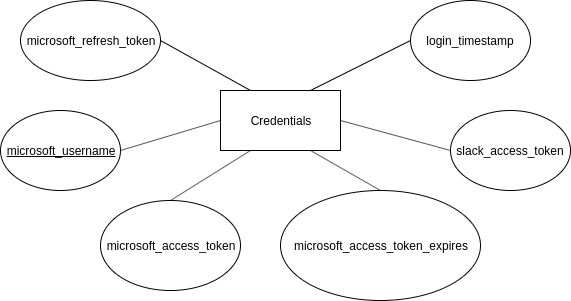
\includegraphics[width=10cm]{./Gambar/ERD.png}
  \centering
  \caption{ER Diagram untuk tabel Credentials.}
  \label{fig:erd}
\end{figure}
Pada program ini, digunakan 1 tabel basis data yang berfungsi untuk menampung data kredensial dari pengguna yang sudah melakukan \textit{login} dan sudah memberikan izin terhadap program ini untuk mengakses \textit{Microsoft Graph} dan \textit{Slack}-nya. Tabel tersebut diberi nama \textit{Credentials}. Kolom yang terdapat pada tabel basis data ini antara lain:
\begin{itemize}
    \item microsoft\_username(TEXT)
    Kolom ini berfungsi sebagai \textit{primary key} yang membedakan antara satu pengguna dengan pengguna lainnya. Nilai untuk kolom ini diambil dari nilai yang didapat saat program meminta \textit{access token}. Saat meminta \textit{access token}, \textit{Microsoft Graph} juga mengembalikan \textit{id\_token} yang jika dilakukan \textit{decode} akan berisi data pengguna yang melakukan \textit{login} termasuk data \textit{username} yang dipakai oleh pengguna. 
    \item microsoft\_refresh\_token(TEXT)
    Kolom ini berfungsi untuk menampung \textit{refresh token} yang didapat saat melakukan \textit{request} ke \textit{Microsoft Graph} yang digunakan untuk melakukan \textit{request} ulang \textit{access token} setelah \textit{access token} sebelumnya kadaluarsa. 
    \item microsoft\_access\_token\_expires(INTEGER)
    Kolom ini berfungsi untuk menampung lamanya masa \textit{access token} akan berlaku. Nilai ini didapat saat awal melakukan \textit{request} \textit{access token} dengan mengambil nilai \textit{expires\_in} dari respon yang didapat. 
    \item microsoft\_access\_token(TEXT)
    Kolom ini berfungsi untuk menampung \textit{access token Microsoft Graph} yang didapat dari \textit{request}. 
    \item slack\_access\_token(TEXT)
    Kolom ini berfungsi untuk menampung \textit{access token Slack} yang didapat dari \textit{request}. 
    \item login\_timestamp(TEXT)
    Kolom ini berfungsi untuk menampung waktu saat pengguna melakukan \textit{login}. 
\end{itemize}

\section{Perancangan Antarmuka}
\subsection{\textit{Route} /}
Pada route ini, antarmuka yang dirancang akan seperti pada gambar \ref{fig:mockup_halaman_awal}. Di dalam perancangan antarmuka route ini akan memiliki sebuah tulisan yang berisi penjelasan fungsi dan mengarahkan kepada pengguna untuk menggunakan perangkat lunak ini. Selain ada sebuah tulisan untuk petunjuk, di dalam halaman ini juga terdapat sebuah tombol yang akan membawa pengguna untuk melakukan login kepada Windows Live dan perangkat lunak ini akan mencatat access token yang didapat dari Windows Live dan segala data yang diperlukan. 

\begin{figure}[h]
  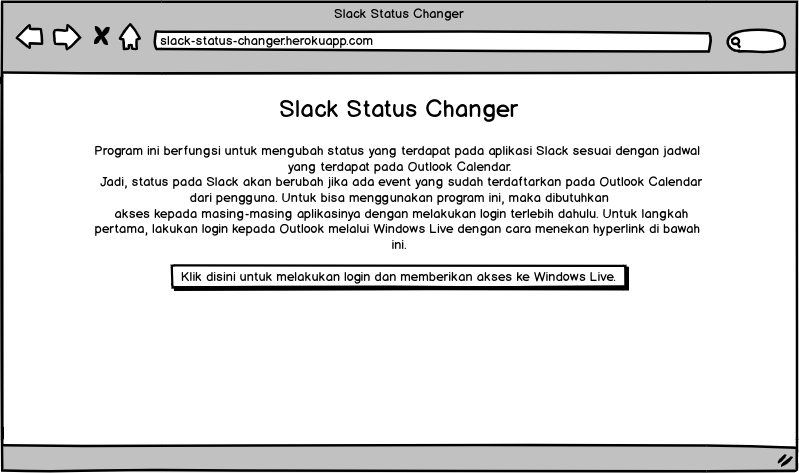
\includegraphics[width=10cm]{./Gambar/MockUp/Step1.png}
  \centering
  \caption{Rancangan antarmuka halaman awal.}
  \label{fig:mockup_halaman_awal}
\end{figure}

\subsection{\textit{Route} /authorize}
Pada route ini, antarmuka yang dirancang seperti pada gambar \ref{fig:mockup_halaman_kedua}. Di dalam perancangan antarmuka route ini akan ada sebuah tulisan lagi yang membantu mengarahkan pengguna untuk melakukan langkah selanjutnya agar bisa memakai perangkat lunak ini dengan baik. Lalu di dalam perancangan ini juga terdapat sebuah tombol yang mengarahkan pengguna melakukan langkah selanjutnya yaitu melakukan login ke aplikasi Slack. Tombol itu juga akan membawa pengguna ke antarmuka dari Slack untuk melakukan login. 

\begin{figure}[h]
  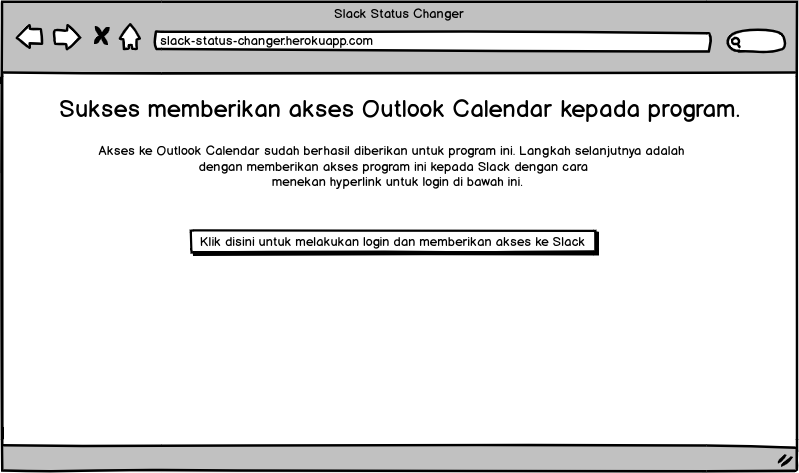
\includegraphics[width=10cm]{./Gambar/MockUp/Step2.png}
  \centering
  \caption{Rancangan antarmuka halaman setelah login Windows Live.}
  \label{fig:mockup_halaman_kedua}
\end{figure}

\subsection{\textit{Route} /slackAuthorize}
Pada route ini, antarmuka yang dirancang seperti pada gambar \ref{fig:mockup_halaman_ketiga}. Di dalam perancangan antarmuka route ini, hanya akan ada sebuah tulisan yang merupakan sebuah pesan bahwa semua langkah yang dijalankan sudah berhasil dan sudah berhasil untuk memakai perangkat lunak ini.  

\begin{figure}[h]
  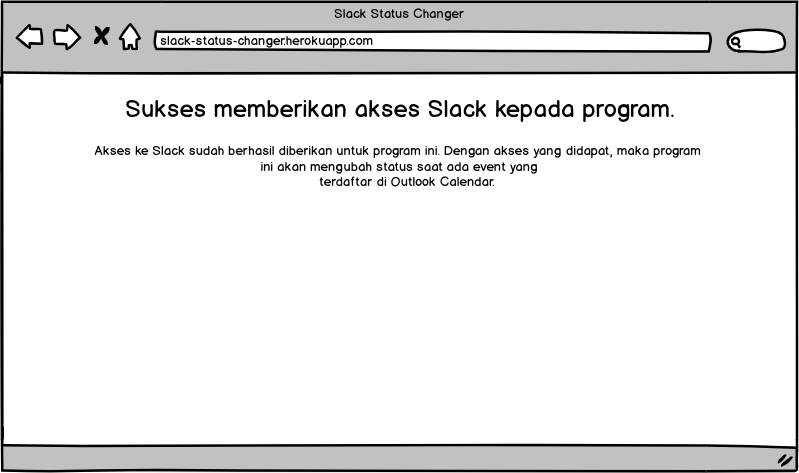
\includegraphics[width=10cm]{./Gambar/MockUp/Step3.png}
  \centering
  \caption{Rancangan antarmuka halaman setelah login Slack.}
  \label{fig:mockup_halaman_ketiga}
\end{figure}

